\documentclass[10pt,twocolumn,letterpaper]{article}

\usepackage{cvpr}
\usepackage{times}
\usepackage{epsfig}
\usepackage{graphicx}
\usepackage{amsmath}
\usepackage{amssymb}

% Include other packages here, before hyperref.

% If you comment hyperref and then uncomment it, you should delete
% egpaper.aux before re-running latex.  (Or just hit 'q' on the first latex
% run, let it finish, and you should be clear).
\usepackage[pagebackref=true,breaklinks=true,letterpaper=true,colorlinks,bookmarks=false]{hyperref}

\cvprfinalcopy % *** Uncomment this line for the final submission

\def\cvprPaperID{****} % *** Enter the CVPR Paper ID here
\def\httilde{\mbox{\tt\raisebox{-.5ex}{\symbol{126}}}}

% Pages are numbered in submission mode, and unnumbered in camera-ready
\ifcvprfinal\pagestyle{empty}\fi
\begin{document}

%%%%%%%%% TITLE
\title{Deep Learning for Computer Vision: Final Project Proposal\\End to End Learning for Visual Navigation}

\author{Ute Schiehlen\\
{\tt\small ute.schiehlen@tum.de}
\and
Natalie Reppekus\\
{\tt\small n.reppekus@tum.de}
\and
Areeb Kamran\\
{\tt\small areeb.kamran@tum.de}
\and
Raymond Chua\\
{\tt\small raymond.chua@tum.de}
}

\maketitle
%\thispagestyle{empty}

%
% Proposal I
%
\section*{Proposal I}
\section{Introduction}
%     Explain your general idea and state the problem you are trying to solve.

%     \subsection{Related Works}
%         \begin{itemize}
%             \item Related and previous work on your topic
%             \item A small overview of the SOTA (state-of-the-art)
%             \item What is new/different in your approach?
%             \item[] $\dots$
%         \end{itemize}
An important component in autonomous vehicles is visual navigation. In this project, we intend to solve this problem using an end to end approach. We propose modeling a video of the front camera of a car as an ordered sequence of frames, with additional motion information in the form of optical flow images computed over adjacent frames to get the steering angle. In addition, to further exploit temporal information, we consider a recurrent neural network that uses {\em Long-Short term memory} (LSTM) cells as our main architecture. 

\section{Related Work}
End to end learning using {\em fully convolutional networks} (FCNs) has proven to be successful in many computer vision tasks such as Recognition\cite{DBLP:journals/corr/SermanetEZMFL13}, Object Detection\cite{DBLP:journals/corr/SermanetEZMFL13}, Localization\cite{DBLP:journals/corr/SermanetEZMFL13, conf/cvpr/OquabBLS15} and Semantic Segmentation \cite{DBLP:journals/pami/ShelhamerLD17}. One reason why end to end learning is so powerful is that it allows the network to learn the internal representation of the data using the provided training information.

In addition, videos are composed with spatial and temporal components. We consider using dense optical flow information from the image sequences as additional data, which has shown to improve results for action recognition\cite{DBLP:conf/nips/SimonyanZ14} and video classification\cite{DBLP:conf/cvpr/NgHVVMT15}. These approaches use a two-stream network, one for spatial information and one for motion. The two streams are then merged to compute a fusion score.

Bojarski et al.\cite{DBLP:journals/corr/BojarskiTDFFGJM16} has shown that end to end learning can also be applied for self-driving cars. They propose a model which consists of one normalization layer, five convolutional layers and three fully-connected layers \cite{DBLP:journals/corr/BojarskiTDFFGJM16}, using only human steering angle as the training signal. The network is able to drive the car autonomously for 90$\%$ and $98\%$ of the time during the simulation and on-road tests respectively \cite{DBLP:journals/corr/BojarskiTDFFGJM16}.

\section{Our Approach}
Although the model from Bojarski et al.\cite{DBLP:journals/corr/BojarskiTDFFGJM16} has achieved successful results, it did not fully exploit the temporal information of the image sequences. The network is trained with each sample being a single frame from the video. Since the frames are highly dependent, we believe that results can be greatly improved if this is taken into consideration by a network. As such, we consider a model that is capable of learning long-term dependencies. One such network architecture is {\em Long Short Term Memory} (LSTM)\cite{DBLP:journals/neco/HochreiterS97}, which is a variant of {\em Recurrent Neural Network} (RNN). 

We would like to compare the network described in\cite{DBLP:journals/corr/BojarskiTDFFGJM16} with a network consisting of a few convolutional blocks based on {\em Residual Networks}\cite{He2015} (ResNet), whose output is fed into the LSTM network. If this yields promising results we will extend this architecture by adding another convolutional network which takes optical flow data generated from the image sequences as input. Its output will be concatenated with the output of the convolutional network from before and used as input for the LSTM network.


\section{Dataset}          
We consider using the open dataset provided by Udacity\cite{udacityDataset}, more specifically the CH2$\_$002 training dataset from the second challenge. It contains six different recordings of driving scenarios with a total of approx. 28 minutes. The first one, for example, is recorded in direct sunlight with many lightning changes on a divided highway including turns in the beginning and a lane merge at the end and has a duration of 221 seconds.

We will split this dataset into train, validation and test set with a 60$\%$, 20$\%$, 20$\%$ distribution respectively. The JPG images will be used as the input source to our network and the steering wheel angel as the corresponding labels. As stated in the README of this project, the data is a cleaned version complying with the defined naming schema and is supposed to be error free.

% \begin{itemize}
% \item https://github.com/udacity/self-driving-car/tree/master/datasets
% \item https://docs.google.com/document/d/1HM0CSmjO8nOpUeTvmPjopcBcVCk7KXvLUuiZFS6TWSg/pub
% \end{itemize}

%     \begin{itemize}
%         \item Are you working with an existing dataset or is data collection part of your project?
%         \item Explain the general nature of your data (show examples if beneficial)
%         \item Does your data provide the labels necessary for training?
%         \item Explain possible problems with the dataset
%         \item What are your inputs and outputs?
%         \item[] $\dots$
%     \end{itemize}

\section{Methodology}
\subsection{Network Architecture}
%    Describe all the different phases/components/steps on how you are planning to solve your previously stated problem. Try to give us a clear picture of your methodology and remember that the project's focus is on deep learning. Try to elaborate on the following points:
%    \begin{itemize}
%        \item Network architecture(s)
%        \item Transfer learning and training from scratch
%        \item Resource management (please consider GPU memory)
%        \item[] $\dots$
%    \end{itemize}
 Due to the nature of the problem, there might be a high number of frames where the car is just going straight, which results in minimal steering angles. In order to have a uniformly  distributed dataset, we split the dataset into multiple bins, based on the steering angles. We can then consider a subset of the training data, such that all the bins are equally represented. 
 
 \begin{figure} [ht]
 	\centering
 	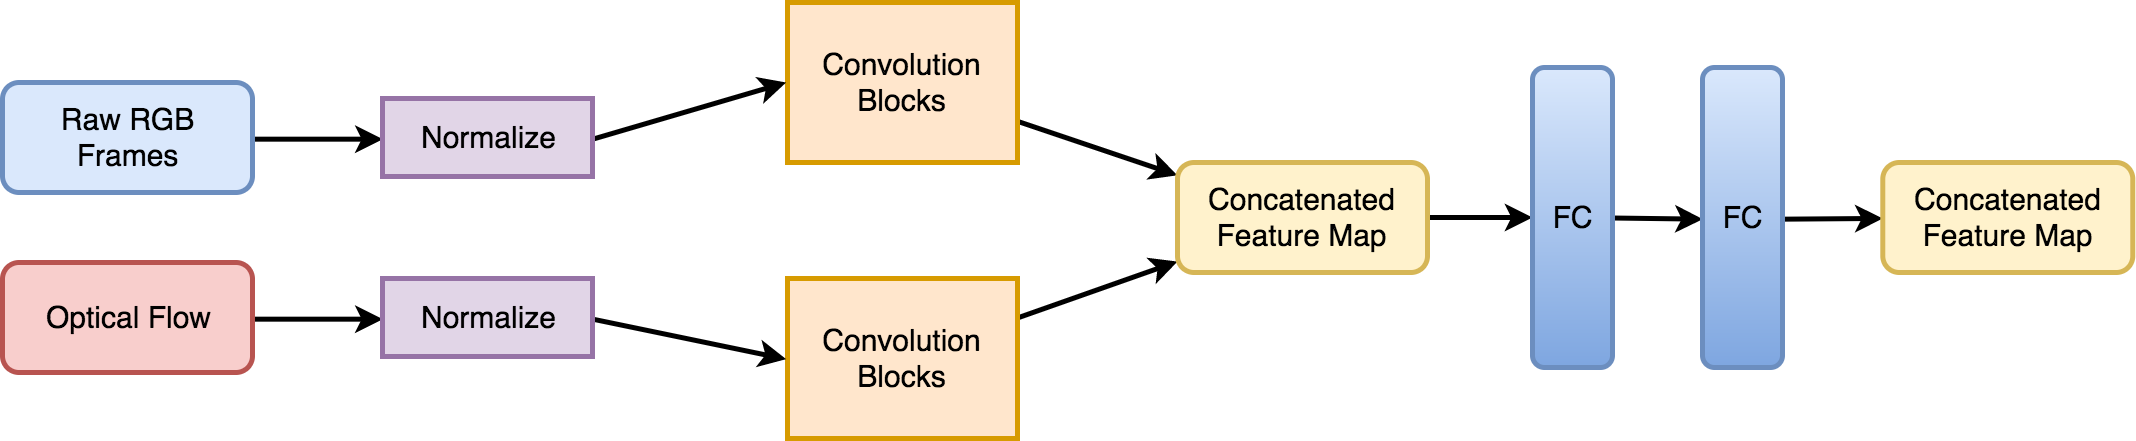
\includegraphics[scale=0.11]{conv_network}
 	\caption{Convolutional Network for our Image Sequences and Optical Flow. Best view in color.}
 	\label{fig:convNet}
 \end{figure}
 
 
 Using this new dataset, for our final network we can consider each training sample as a pair of a RGB image and its corresponding optical flow data for each time step. The training sample is normalized separately. We can then feed the normalized data into our convolutional network for feature extraction which results in a concatenated feature map (Figure. \ref{fig:convNet}).
 
 
  \begin{figure} [ht]
 	\centering
 	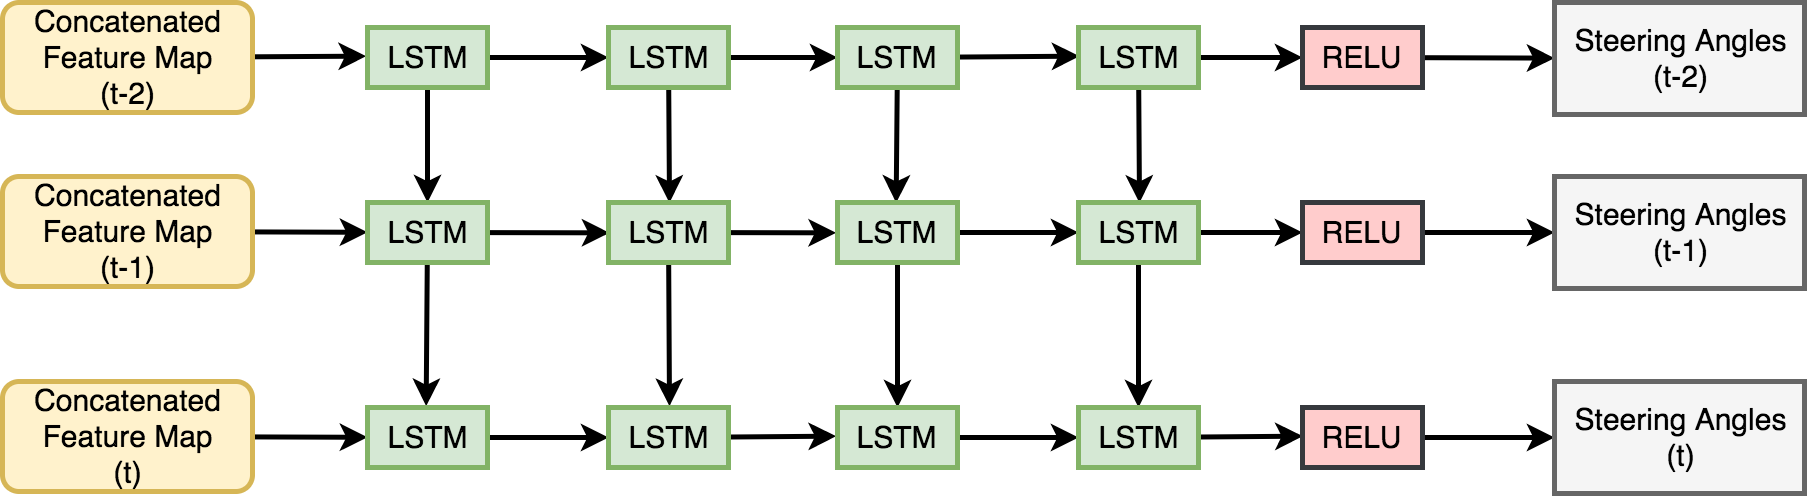
\includegraphics[scale=0.13]{lstm_network}
 	\caption{Long-Short Term Memory Network. Inputs are the concatenated feature maps generated for each time step. A rectified linear (RELU) activation layer is applied at the end. Best view in color.}
 	\label{fig:lstmNet}
 \end{figure}

We feed the concatenated feature map into four stacked LSTM layers. A rectified linear activation layer is added to predict the steering angles for each time step. (Figure. \ref{fig:lstmNet}). 

We consider $\boldsymbol{\theta} \in \mathbb{R}^d$ as the set of our network parameters, $\mathbf{x}  = (x_1, ..., x_t)$ as our RGB image sequence input and $\mathbf{o} = (o_1, ..., o_t)$ as our Optical Flow sequence input. By denoting $f$ as our network and $\mathnormal{y}$ as the ground truth steering angle per frame, we define our loss function based on the \textbf{Mean Square Error} metric (MSE) : 
\begin{align}
\mathnormal{Losst} = \frac{1}{2}\bigg( f(\hat{y}; \mathbf{x}, \mathbf{o}, \boldsymbol{\theta}) - \mathnormal{y} \bigg)^{2} + \frac{\lambda}{2}\mid \mid \boldsymbol{\theta} \mid \mid ^2
\label{eq:loss}
\end{align}
where $\hat{y}$ is our predicted steering angle and $\lambda$ is our regularization parameter. 

\subsection{Transfer learning and training from scratch}
As described in methodology, the first two parts of our approach are based on transfer learning. In the first part we build the network based on\cite{DBLP:journals/corr/BojarskiTDFFGJM16}. In the second part, we use our trained model from the first part and train the the LSTM layers on top. For the optical flow integration, we only use the pre-trained convolutional layers and train the new convolutional and LSTM layers from scratch.

\subsection{Resource management}
For development our personal or chair machines are used and the network is trained via AWS services.

\section{Outcome}
%    What is your desired outcome or aspiration for the project?
We hope to to train the network successfully. By using Bojarski et al.\cite{DBLP:journals/corr/BojarskiTDFFGJM16} model as the baseline, the project can be considered a success if there are any improvements to the prediction results.

%
% Proposal II
%
\section*{Proposal II}
\setcounter{section}{0}
\section{Introduction}
In the project we propose to predict the number of crimes in a city. This is a phenomenon which depends on both space and time. However training neuronal network architecture directly on this data would not be feasible. So from the crime data, we propose to build point cloud maps for the city of San Francisco. Each point map can be of a range between just one hour and one day. That way we can generate images for about 10 years from the data available. 

\section{Our Approach}
We are proposing to first generate point clouds or dot map images from data and then train two networks on it. The data itself is available from 2003 to 2017 and can be divided into training data which can be first 12 years and test data which would be the next 3 years. 

\section{Methodology}
Our methodology is to use two networks and use majority voting for final prediction. One network would deal with a temporal information (time series only) and would be an LSTM network. The other network would work with spatial data and information (coordinates) and so would be a convolutional network. We then would combine the results from both for predicting when and where might a crime be expected in a city.

\section{Dataset}          
We would use the open Data set from City of San Francisco's open data portal \cite{SFopendata}. It has detailed crime data which can be broken down into multiple categories as well (robbery, manslaughter, auto theft, etc)

{\small
\bibliographystyle{ieee}
\bibliography{bib}
}

\end{document}
